% SAMBP Inverse Estimation Diagram
% Compile with: pdflatex inverse_estimation_diagram.tex

\documentclass{standalone}
\usepackage{tikz}
\usetikzlibrary{shapes,arrows,positioning}

\begin{document}
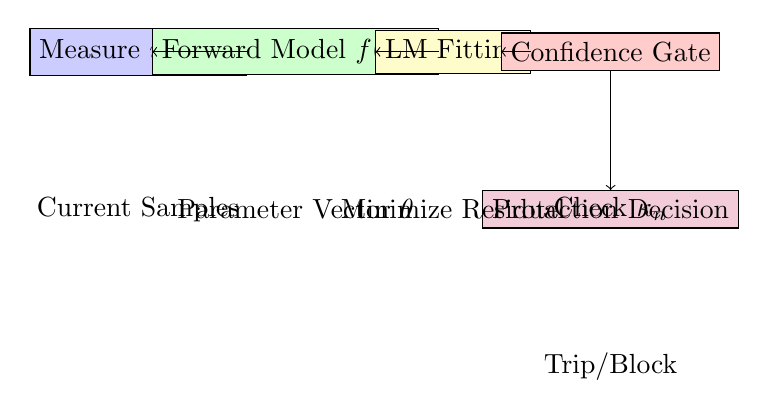
\begin{tikzpicture}[node distance=2cm, auto]
    % Nodes
    \node [draw, rectangle, fill=blue!20] (measure) {Measure $i_{diff}(t)$};
    \node [draw, rectangle, fill=green!20, right of=measure] (model) {Forward Model $f(\boldsymbol{\theta}, t)$};
    \node [draw, rectangle, fill=yellow!20, right of=model] (fit) {LM Fitting};
    \node [draw, rectangle, fill=red!20, right of=fit] (confidence) {Confidence Gate};
    \node [draw, rectangle, fill=purple!20, below of=confidence] (decide) {Protection Decision};

    % Arrows
    \draw [->] (measure) -- (model);
    \draw [->] (model) -- (fit);
    \draw [->] (fit) -- (confidence);
    \draw [->] (confidence) -- (decide);

    % Labels
    \node [below of=measure] {Current Samples};
    \node [below of=model] {Parameter Vector $\boldsymbol{\theta}$};
    \node [below of=fit] {Minimize Residual};
    \node [below of=confidence] {Check $\kappa_n$};
    \node [below of=decide] {Trip/Block};
\end{tikzpicture}
\end{document}